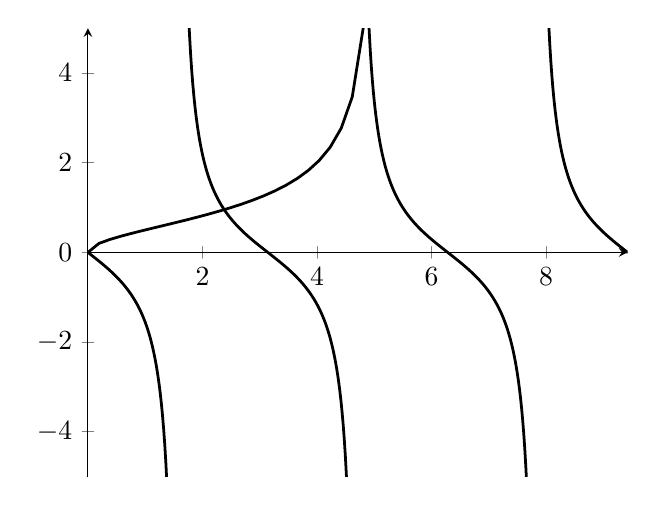
\begin{tikzpicture}[cap=round,>=latex]
	\begin{axis}[grid=none,
	axis x line=middle,
	axis y line=left,	
	%enlargelimits,
	%xtick={-1,0,1},
	%xticklabels={$-a$, $0$, $a$},
	%ytick={1},
	%yticklabels={$U_0$},
	%domain=0:700
	xmin=0,
	xmax=3*pi,
	ymin=-5,
	ymax=5,
	restrict y to domain=-10:10 
	]
	
	\addplot[no markers, line width=1, samples=50, domain=0:3*pi] {sqrt(x/( 5-x))};
	\addplot[no markers, line width=1, samples=500, domain=0:3*pi] {-tan(deg(x))};	
	\end{axis}								
\end{tikzpicture}